


\subsection{Beacon Vendors}

I have decided to use the iBeacon technology pioneered by Apple as
the underlying technology for my project. This iBeacon technology has been harnesed by companies and used in a variety of ways. The most popular use found for the iBeacon techonology is to create small hardware beacons, which are used in retail shops for GeoFencing. It has been used to give targeted advertisement to users and customers.

Beekn\cite{beekn} is a website that has accumulated a lot of information about iBeacons. Beekn have reviewed a lot of vendors who provide good iBeacon technology. In this section I will look at the main vendors I have
considered and also the Intel Gallileo chip which is a more powerful chip.


\subsubsection{Qualcomm}

Qualcomm\cite{quallcomm} is one of the biggest chip manufacturing
companies. They are a world leader in 3G and next generation mobile
technologies. Naturally they have also launched their brand of beacons
called Gimbal\cite{gimbal}. The Gimbal beacons are relatively cheap
around \$5 when bought in bulk. However the main advantage is the
robust back-end system and SDK. Gimbal was launched in 2 sizes:

\begin{figure}[H]
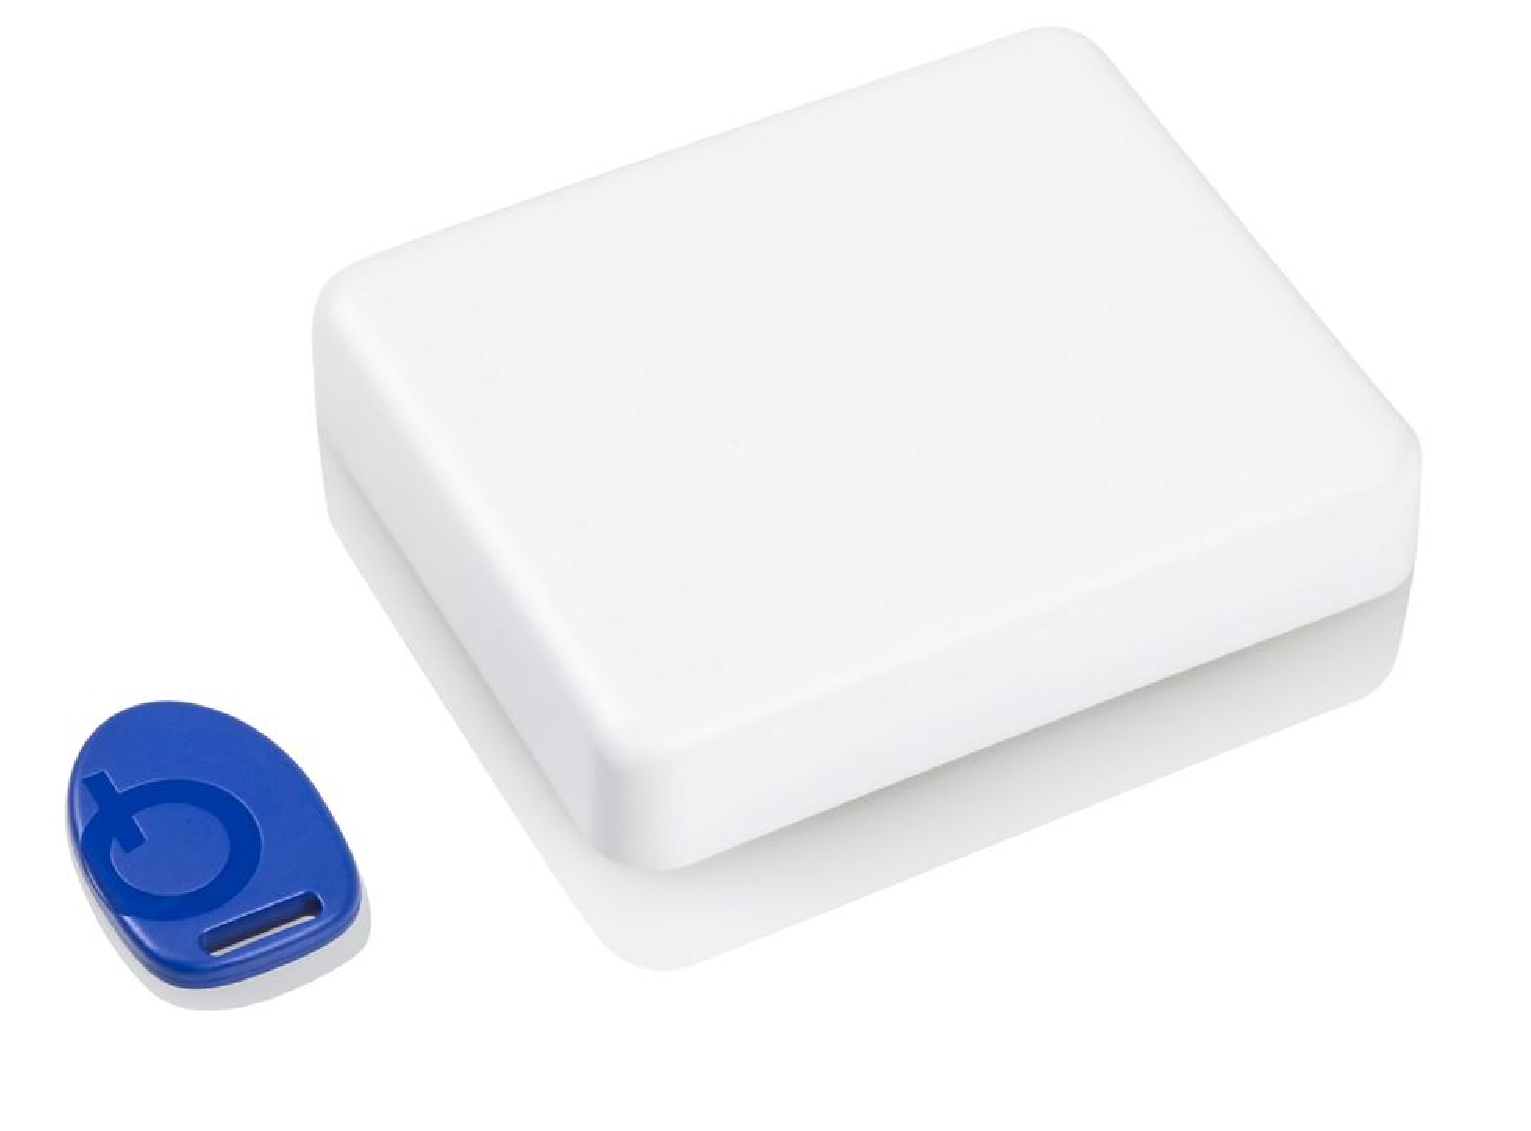
\includegraphics[scale=0.3]{images/gimbal-beacon}

\protect\caption{Gimbal Beacons}
\end{figure}

\begin{enumerate}
\item Series 10: Comes in a small size, (28x40x5.6mm), and designed with
a loop to enable more applications. The battery life is around
3 months and transmission rate of twice per second. It also has a
temperature sensor on it.
\item Series 20: Comes in a bigger size, size of a playing card. It is also
more robust than the series 10. It uses replaceable AA alkaline battery
giving it more battery life and also a higher transmission rate. Sends more packets per second.
\end{enumerate}
More than the size and robustness of the beacons, the factor that
sets Gimbal apart from its competitors is its back-end system. Gimbal
is shipped with a full functioning back-end system that supports Geo-fencing\cite{geofencing},
analytical, communication and application management tools. They have
also introduced features which allow developers to set up rules
for entering and exiting the beacon proximity.


\subsubsection{Estimote}

Estimote\cite{estimote} is an upcoming start up that has made waves
in the beacon technology market. Having sold over 40,000 developer
kits since its launch in 2013, it is one of the biggest vendors for
beacons enjoying a large market share. Similar to the Gimbal they
also provide two sizes. However the Estimote beacons are relatively
more expensive than the Gimbal.
\begin{enumerate}
\item The main product is called the Estimote Beacon which is quite a large
device. It's main role, is to be stationary stuck onto a wall somewhere
i.e in a supermarket, for Geo-fence it to give targeted advertisement
to the users depending on the location.  
\item They have also recently brought out another product called Estimote
Stickers. Which is more like a rival to the Gimbal series 10, its
a smaller version of the beacon which can potentially turn any device
into a nearable. It also has sensors such as accelerometer and
temperature feedback to give a more detailed information on the activity and
the location of the device it's stuck onto.
\begin{figure}[H]
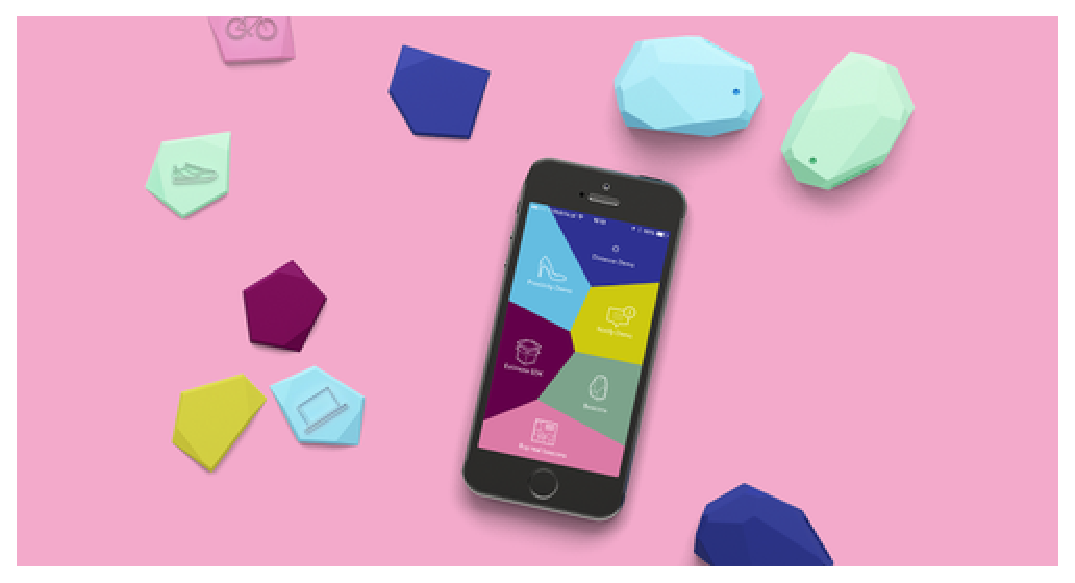
\includegraphics[scale=0.3]{images/estimote}

\protect\caption{Estimote beacons}


\end{figure}

\end{enumerate}

\subsubsection{Intel Edison}

Intel Edison\cite{intel-edision} is a tiny computer offered by Intel
as a development system for wearable devices. It has a high performance
dual core CPU with integrated Wi-Fi and BLE, all using very low power, allowing it to have all the capabilities of a computer but with a longer battery
life and more portability. It is one of the main components used in
Internet of Things (IoT). It has access to device-to-device and device-to-cloud
connectivity framework enabling cross device communication and a
cloud based, multi-tenant, time-series analytical service\cite{intel-edison}. Since it
is a highly powerful machine with both Wi-fi and BLE support, its
an ideal candidate for the beacons I need for my research. However
due to its relatively low battery life (around 1 day) and the having
more power and facilities than I need, I have not used the Edison.


\begin{figure}[H]
\includegraphics{images/intel-edison-560}
\protect\caption{Intel Edison}
\end{figure}


